\documentclass[11pt,letterpaper]{article}

\usepackage{graphicx}
\usepackage[margin=1in]{geometry}
\usepackage[T1]{fontenc}
\usepackage[utf8]{inputenc}
\usepackage{authblk}
\usepackage{fancyhdr}
\usepackage{lastpage}
\usepackage[parfill]{parskip}
\usepackage{subcaption}

\pagestyle{fancyplain}
\fancyhf{}
\fancyfoot[R]{\footnotesize Page \thepage\ of \pageref{LastPage}}

\renewcommand{\headrulewidth}{0.0pt} % No header rule
\renewcommand{\footrulewidth}{0.4pt} % Thin footer rule

\begin{document}

\title{Fastlife: Parallelizing the Game of Life with MPI}
\author[ ]{Benjamin Bengfort}
\affil[ ]{Department of Computer Science}
\affil[ ]{University of Maryland}
\affil[ ]{\textit{<bengfort@cs.umd.edu>}}

\date{October 6, 2015}

\maketitle

Conway's Game of Life is a two dimensional cellular automaton whose evolution over time is determined by its initial state. For every time step in the simulation, a new state is computed for each individual cell based on the neighborhood of their surrounding cells. In a single processor (sequential) version of this computation, the entire simulation matrix must be iterated upon to create a new state with those computed values. However, as the computation for each cell depends solely on the local cells surrounding it, the simulation is a good candidate for parallelism, such that multiple processors simultaneously compute the new state for smaller, independent regions of the simulation.

In this brief report I present \texttt{fastlife}, a parallel implementation of Life modeled as a distributed memory system using message passing via the Open MPI library. \texttt{fastlife} uses a columnar decomposition to partition the simulation region across multiple processors, minimizes message traffic, and has attempted load balance the work among all nodes. Using these techniques \texttt{fastlife} improves the performance of the Life simulation by using 16 processors instead of a single one. The rest of the paper describes the decomposition methodology, the attempts at load balancing, as well as the performance results.

\section*{Decomposition}

The domain of our version of the Life simulation is a finite two-dimensional array, whose bounds are given as input to the program. I used a columnar decomposition methodology to evenly partition the input space across the number of available processors such that all columns are equal except for the last column, which may be the same size or \textit{smaller} than the rest of the partitions. This is in contrast to an integer division method of partitioning, which leaves the last column larger in the case of a remainder. My preference was for more, slightly larger columns rather than one extra large column.

Each partition contained left and right ghost columns that needed to be synchronized with neighbor partitions after each generation of the simulation. This resulted in a two stage update process shown in Figure \ref{fig:columnar_decomposition}, where at the conclusion of computing the next state in the simulation, each partition $n_i$ would send its right ghost column to the neighbor with rank $n_{i+1}$, then would listen for a message from its neighbor $n_{i-1}$ -- updating its left ghost column with the result. Then the process would reverse, each node sending its left ghost column and updating its right.

\begin{figure}
	\centering
    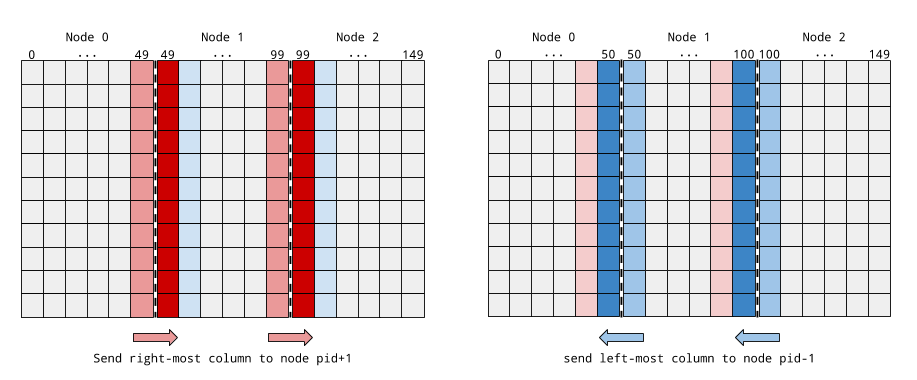
\includegraphics[width=\textwidth]{figures/columnar_decomposition.png}
    \caption{\textsf{Fastlife uses a 2D columnar decomposition for parallelization. Synchronization between partitions requires a two-phase ghost column transfer. First, all partitions send their right ghost column and update their left; then all partitions send their left and update their right. The two phase ghosting without barriers allows computation to continue even while message passing is occurring.}}
    \label{fig:columnar_decomposition}
\end{figure}

The number of messages are minimized by packing the entire column into a single message rather than sending each cell at a time. The number of messages per generation is therefore dependent on the number of partitions, namely $2n-2$ where $n$ is the number of partitions. However, I would note that as the message size increases (e.g. as the number of rows in the simulation increases), messages may need to be chunked by a fixed size. Another solution would be to send an array of only the positions in the column that were occupied, thus reducing the message size, but not necessarily the number of messages.

During any given generation, each node could either be updating the simulation, or performing right or left ghosting. No synchronization occurs during any of these phases, therefore processes can continue processing even while message passing is occurring. However, in order to conclude a single generation, all processes had to reach a \texttt{MPI\_Barrier}. After the barrier, a rebalance phase was applied in order to attempt load balancing, thus ensuring that all nodes were processing the same generation without duplication.

\section*{Load Balancing}

After the generation computation, ghosting, and synchronization, a rebalance phase could be applied to load balance the computation. Unfortunately at the time of this writing I was unable to implement a rebalancing that improved the parallel performance. I attempted two methods; first, shifting the partition boundaries so that each partition was smaller but covered only the location where occupied cells existed, and second, using more partitions than nodes.

In the first case, I observed that much of the simulation world had little computation being applied to it since the cells there were empty. In order to reduce the computational space, I had each node keep track of the right most column where cells were occupied during their update computation. During the rebalance phase, an \texttt{MPI\_Allreduce} was used to compute the \texttt{MPI\_MAX} of these columns -- the farthest right extent to which the world existed at that stage of the computation. I then rebalanced the partitions such that each node only operated over an occupied region, with enough buffer space such that the world could grow. However, in order to make this work, scatter/gather operations were required to also rebalance the memory of each node; this resulted in more messages and a reduction in performance.

My second attempt was to use more partitions than nodes, with the idea that nodes could compute the simulation state of a second partition while message passing was occurring. In particular, I divided each partition into two, computing upon the right half of the partition, sending the right ghost column synchronization message and then computing the left half and sending the left column. However, the two stage ghosting protocol already allowed for computation to occur during message passing and this more complex partitioning scheme resulted in an incorrect result.

For larger inputs I believe that these load balancing mechanisms would impact the speed of computation. However, for the size of input that we experimented upon, the additional message passing overhead actually made the computation slower.

\section*{Results}

\begin{figure}
	\centering
    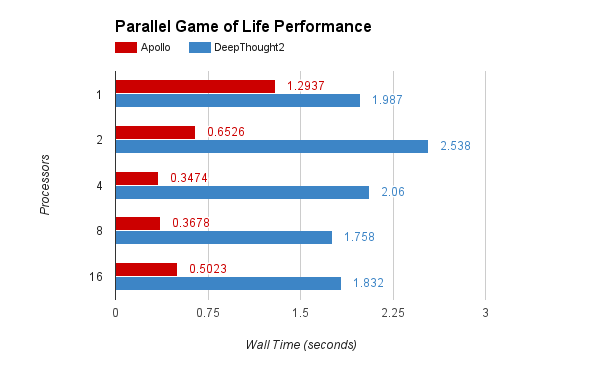
\includegraphics[width=0.7\textwidth]{figures/2d_performance.png}
    \caption{\textsf{Average wall clock times in seconds for 10 fastlife runs of 1, 2, 4, 8, and 16 processors on my MacBook Pro (Apollo) and Deepthought2. On both machines parallelization improves performance.}}
    \label{fig:2d_performance}
\end{figure}

The performance of \texttt{fastlife} was measured on two machines: a MacBook Pro with a 2.8 GHz Intel Core i7 processor with four physical cores and 8 logical ones, and Deepthought2, the University of Maryland's high performance computing cluster with 460 homogenous nodes and approximately 9,280 physical cores. Experimental runs for 1, 2, 4, 8, and 16 processors were timed using the Unix \texttt{time} command (note that on Deepthought2 the \texttt{/usr/bin/time} command was used not the TCSH \texttt{time} utility). Each experiment for a processors/machine pair consisted of 10 runs, where half the runs were delayed 2 hours (to prevent variable performance due to other jobs on the machine). The average real time (wall clock time) for each of the ten runs is given in Figure \ref{fig:2d_performance}.

The \texttt{fastlife} implementation did benefit from a performance improvement in parallelism from 1 core to 16 cores on both Apollo and Deepthought2, although the more dramatic improvement was seen on Apollo. I attribute this to the fact that no network connection was required on Apollo (the timing of Deepthought2 includes the time required to move the job from the login node to the compute cluster and retrieve the output). It is also interesting to note that 8 processors is the limit of Apollo's timing gain, probably directly related to the number of logical cores that exist on the machine. Interestingly, the message passing overhead on Deepthought2 means that the performance between 1 and 4 cores is approximately the same, it is only after 4 cores that performance benefits of parallelism are shown.

\begin{figure}[h]
	\centering
	\begin{subfigure}{0.49\textwidth}
		\centering
		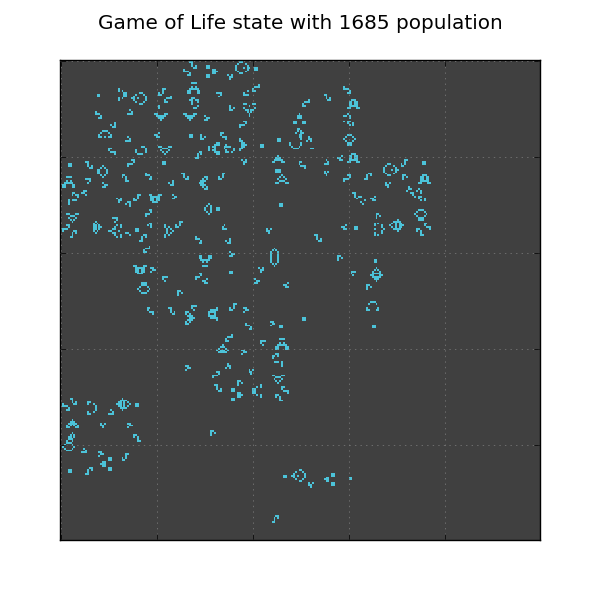
\includegraphics[width=\textwidth]{figures/initial_state.png}
		\caption{\textsf{Initial simulation state of final.data}}
        \label{fig:initial_state}
	\end{subfigure} \hfill
	\begin{subfigure}{0.49\textwidth}
		\centering
		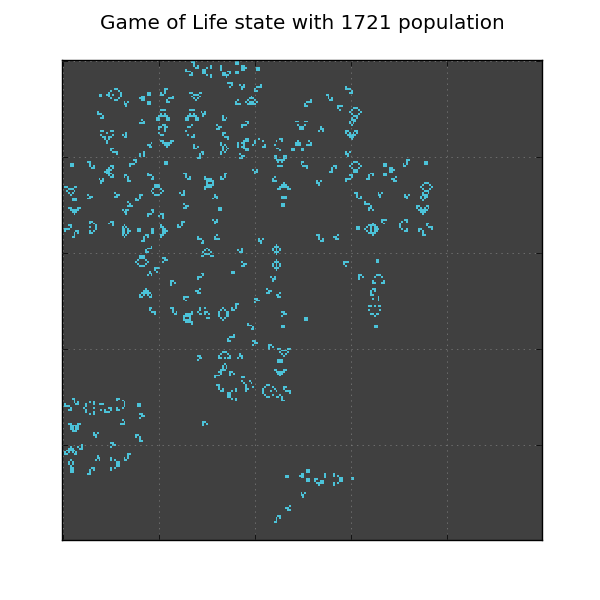
\includegraphics[width=\textwidth]{figures/final_state.png}
		\caption{\textsf{Final simulation state after 500 generations}}
        \label{fig:final_state}
	\end{subfigure}
    \caption{\textsf{Game of Life simulation output visualized using Python and matplotlib.}}
    \label{fig:centrality}
\end{figure}

\section*{Discussion}

Programming with distributed memory parallelism and Open MPI requires the programmer to consider the cost of message passing as the primary time cost to parallelism. This leads to a design focus on decomposition of the problem space and load balancing, and it is very easy to reduce the performance of a parallel version over a sequential one because of networking costs. However, the MPI interface is straight forward and easy to use with primitives for a variety of essential communication operations, making the implementation details straight forward, and allowing the programmer to focus on the parallel design of an algorithm.

\bibliographystyle{plain}
\bibliography{paper}

\newpage
\appendix

\begin{table}[t!]
    \renewcommand{\arraystretch}{1.5}
    \centering
\begin{tabular}{ | c || c | c | c | c | c | }
	\hline
	\textbf{Run #} & \textbf{1 Node} & \textbf{2 Nodes} & \textbf{4 Nodes} &	 \textbf{8 Nodes} & \textbf{16 Nodes} \\
	\hline
	1 & 1.254 & 0.631 & 0.34 & 0.356 & 0.498 \\
	2 & 1.3 & 0.648 & 0.344 & 0.375 & 0.491 \\
	3 & 1.322 & 0.665 & 0.352 & 0.371 & 0.491 \\
	4 & 1.207 & 0.652 & 0.348 & 0.365 & 0.493 \\
	5 & 1.263 & 0.665 & 0.347 & 0.374 & 0.527 \\
	6 & 1.342 & 0.635 & 0.346 & 0.375 & 0.518 \\
	7 & 1.323 & 0.673 & 0.361 & 0.381 & 0.51 \\
	8 & 1.262 & 0.634 & 0.335 & 0.352 & 0.493 \\
	9 & 1.353 & 0.672 & 0.361 & 0.356 & 0.502 \\
	10 & 1.311 & 0.651 & 0.34 & 0.373 & 0.5 \\
	\hline
	\textbf{Mean} & 1.2937 & 0.6526 & 0.3474 & 0.3678 & 0.5023 \\
	\hline
\end{tabular}
	\caption{Performance of Fastlife on Apollo}
	\label{table:apollo-performance}
\end{table}

\begin{table}[t!]
    \renewcommand{\arraystretch}{1.5}
    \centering
\begin{tabular}{ | c || c | c | c | c | c | }
	\hline
	\textbf{Run #} & \textbf{1 Node} & \textbf{2 Nodes} & \textbf{4 Nodes} &	 \textbf{8 Nodes} & \textbf{16 Nodes} \\
	\hline
	1 & 2.1 & 2.75 & 1.98 & 1.74 & 1.95 \\
	2 & 2.35 & 2.23 & 2.11 & 1.72 & 1.92 \\
	3 & 1.98 & 2.39 & 2.11 & 1.84 & 1.95 \\
	4 & 1.95 & 2.97 & 2.07 & 1.74 & 1.93 \\
	5 & 1.89 & 2.59 & 2.14 & 1.81 & 1.83 \\
	6 & 1.87 & 2.39 & 2.06 & 1.78 & 1.68 \\
	7 & 1.81 & 2.73 & 1.92 & 1.7 & 1.7 \\
	8 & 2.02 & 2.49 & 2 & 1.77 & 1.73 \\
	9 & 2.02 & 2.42 & 2.05 & 1.79 & 1.71 \\
	10 & 1.88 & 2.42 & 2.16 & 1.69 & 1.92 \\
	\hline
	\textbf{Mean} & 1.987 & 2.538 & 2.06 & 1.758 & 1.832 \\
	\hline
\end{tabular}
	\caption{Performance of Fastlife on Deepthought2}
	\label{table:deepthought2-performance}
\end{table}


\end{document}
